\chapter{Analysis}\label{analysis}
\lhead[\fancyplain{}{\bfseries\thepage}]{\fancyplain{}{\bfseries\rightmark}}

In this Chapter we explain the starting implementation and analysis of the model following biological considerations.

\section{Implementation}

The theoretical model has benn analyzed making simulations using Python.
The first thing was to create a class \emph{Random Network} to have a random boolean graph as an object, with its nodes and links, represented by a boolean adjacency matrix.

Every random network is a directed graph and is built to avoid self-loops, this averages to create a random, boolean, and non-symmetric adjacency matrix with null trace.

The first thing to evaluate was to choose the average number of incoming links for each RBN. In Figure \ref{fig:K} we can see that the average discrete evolution of $100$ different realizations of RBNs, with increasing size.
\begin{figure}[h]
\centering
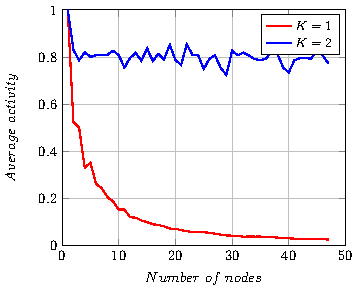
\includegraphics[scale=1.5]{images/K.pdf}
\caption{\emph{Plot of the average activity of the nodes with network of increasing size.
In the case of $K=1$ (i.e. the average number of incoming link for each network is one), the average activity decreases exponentially with the size of the network; in the case of $K=2$ instead, the average activity of the nodes remains stable with the network size.}}
\label{fig:K}
\end{figure}
In the case of $K=1$, i.e. the average number of incoming links for each network is one, the average activity decreases exponentially with the size of the network; in the case of $K=2$ instead, the average activity of the nodes remains stable with networks of increasing size. For this reason, the network considered for this model will take the parameter K constant: $K=2$.
Moreover, we can analyze the average number of outgoing links depending on the network size: In Figure \ref{fig:outgoing}, we can see that the average number of outgoing links tends to the parameter $K$.
\begin{figure}[h]
\centering
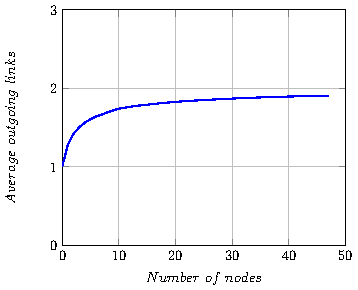
\includegraphics[scale=1.5]{images/outgoing.pdf}
\caption{\emph{Plot of the number of the outgoing links depending on the network size. We can see that the average tends to the parameter $K$. }}
\label{fig:outgoing}
\end{figure}
\section{Discrete evolution}
As shown in Chapter \ref{model}, the discrete time evolution of the network is given by the equation:
$$
\mathnormal{\sigma_i(t+1)=\Theta\biggl(\sum_jA_{ij}\sigma_j(t)\biggr)}
$$
where A is the connectivity matrix of the network.
So this averages that each node which has at least one incoming link with a node which is active, in the next step this node will be active.
At each time step we can measure the average activity of the network, which is the average number of nodes with the value:
$$
\sigma_i(t) = 1
$$


\section{Loops and Control nodes}
In simple random networks one can always find the number of independent loops.
Independent loops determine the complexity of the networks\cite{K38}, and are important for the construction of the model. In fact from the independ loops one can find the \emph{control nodes} of the network, which are the nodes with maximum connectivity. Control nodes determine the whole activity and stability of the network. 
In RBNs with parameter $K=2$, we can see in Figure \ref{fig:loops} that the number of independent loops is linear with the network size.
\begin{figure}[h]
\centering
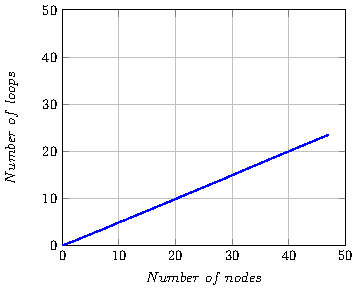
\includegraphics[scale=1.5]{images/loops.pdf}
\caption{\emph{Plot of the number of independet loops in the networks depending on the network size.}}
\label{fig:loops}
\end{figure}



\section{Noise}
The second thing to evaluate is the effect of the noise on the evolution of the network and the difference between noise and parametric noise, where parametric noise refers to the noise which infers in the links and not on the nodes.
To add noise to the system, during the discrete evolution of the network, at each time step there is a probability $p$ for the node or for the link to be turned off.
In Figure \ref{fig:noise} we can see the behavior of the average activity of the network depending on the amount of noise added.
\begin{figure}[h]
\centering
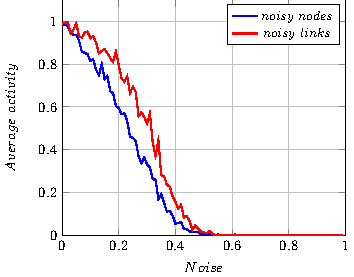
\includegraphics[scale=1.5]{images/noise.pdf}
\caption{\emph{Plot of the effect of the noise on the average activity on the network. In blue the noise works on the nodes on the network, while in red the noise works on the links. Number of nodes for each network: 10; Number of realizations for each value of noise: 100; }}
\label{fig:noise}
\end{figure}
